\documentclass[a4paper]{scrartcl}
\usepackage{scrpage2}
\usepackage[ngerman]{babel}
\usepackage[T1]{fontenc}
\usepackage[utf8]{inputenc}
%\usepackage[pdftex]{graphicx}
%\usepackage[intlimits]{amsmath}
%\usepackage{listings}
%\lstset{frame=single,breaklines=true}
\usepackage{ amssymb }
\usepackage{amsmath}
\usepackage{hyperref}
\usepackage{enumerate}
\usepackage[a4paper, total={19cm, 23cm}]{geometry}
\usepackage{stmaryrd}
\usepackage{esvect}
\usepackage{graphicx}
\pagestyle{scrheadings}
\pagenumbering{gobble}
\ihead{Übungsblatt 5\\Nils Werner 108012219293}
\chead{\\Paul Rösler 108012225686	}
\ohead{Übungsgruppe: Mo. 16:00\\Daniel Teuchert 108012214552}
\setheadsepline{0.4pt}
\begin{document}

\section*{Aufgabe 1}

\newpage
\section*{Aufgabe 2}
\begin{enumerate}[a)]
\item
$R_2, R_3:$\\
$R_2=F_{2\pi 2^{-2}}=F_{\frac{\pi}{2}} = 
\begin{pmatrix}
1 & 0 \\ 0 & e^{\frac{i \pi}{2}} \\
\end{pmatrix} = 
\begin{pmatrix}
1 & 0 \\ 0 & cos(\frac{\pi}{2})+i~sin(\frac{\pi}{2})\\
\end{pmatrix}$ \\
$R_3=F_{\frac{\pi}{4}} = 
\begin{pmatrix}
1 & 0 \\ 0 & e^{\frac{i \pi}{4}} \\
\end{pmatrix} = 
\begin{pmatrix}
1 & 0 \\ 0 & cos(\frac{\pi}{4})+i~sin(\frac{\pi}{4})\\
\end{pmatrix}$ \\
Eigentlich werden kontrollierte $R_k^{-1}$ für die QFT$_{2^n}^{-1}$ benötigt.

\item Für $|z\rangle = |z_1 z_2 z_3\rangle= (\frac{|0\rangle+e^{2\pi i0.x_3} |1\rangle }{\sqrt{2}})\bigotimes(\frac{|0\rangle+e^{2\pi i0.x_2x_3} |1\rangle }{\sqrt{2}})\bigotimes(\frac{|0\rangle+e^{2\pi i0.x_1x_2x_3} |1\rangle }{\sqrt{2}})$ gilt:

\begin{figure}[htp] \centering{
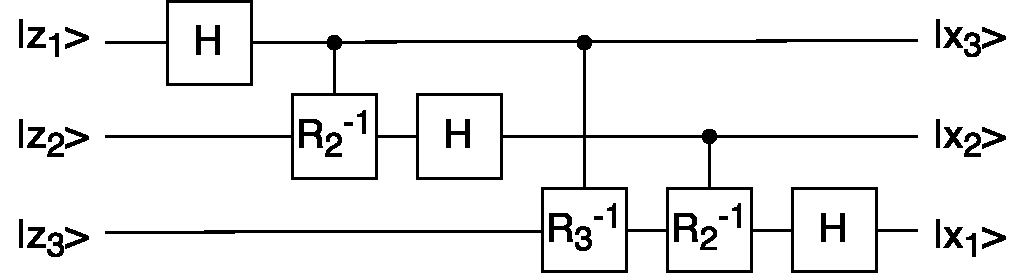
\includegraphics[scale=0.5]{A52b.pdf}}
\caption{Quantenschaltkreis für QFT$_{8}^{-1}$}
\end{figure}


\end{enumerate}

\newpage
\section*{Aufgabe 3}

\newpage
\section*{Aufgabe 4}

\end{document}
